\subsubsection{Фюзеляжная часть центроплана}

Другим проблемным местом была фюзеляжная часть центроплана. Из-за требований компоновки, а именно интеграции двигателя, центроплан необходимо делать изогнутым (Рис.\ref{fig:centroplan}). Это вносит дополнительные трудности в виде увеличения веса по сравнению с прямым центропланом. Исследованию фюзеляжной части центроплана (выделена серым на Рис.\ref{fig:centroplan}) посвящена глава \ref{chap:SolvingModel}.

\begin{figure}[ht]
\centering
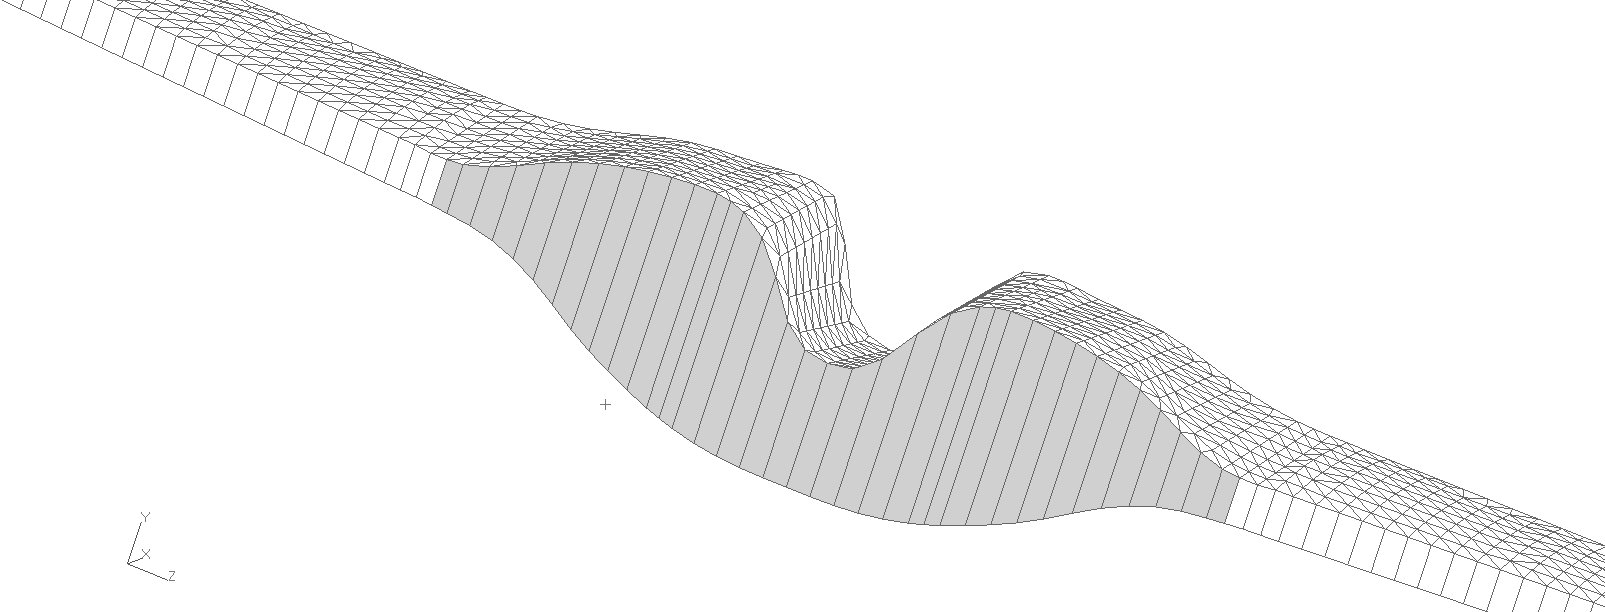
\includegraphics[width=0.6\textwidth]{centroplan}
\caption{Изогнутый центроплан с выделением исследуемой части}
\label{fig:centroplan}
\end{figure}